\section{Video analysis}

video=2D Dims+time Dim


\subsection{Problems: Videos are Big}

数据量太过庞大

SD (640 x 480): ~1.5 GB per minute
HD (1920 x 1080): ~10 GB per minute

Solution: Train on short clips: low fps and low spatial resolution
e.g. T = 16, H=W=112 (3.2 seconds at 5 fps, 588 KB)

\subsection{Video Classification: Single-Frame CNN}

Simple idea: train normal 2D CNN to classify video frames independently!

(Average predicted probs at test-time)

Often a very strong baseline for video classification

在类别差异比较大的时候, 是一个很强的 baseline

\subsection{Video Classification: Late Fusion with FC}

\begin{figure}[htbp]
    \centering
    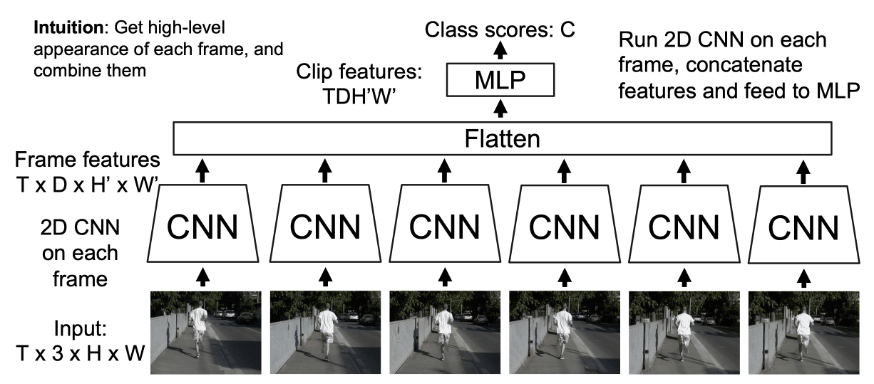
\includegraphics[scale=0.25]{figures/LF_FC.png}
    \caption{Late Fusion with FC}
\end{figure}

看得出来正着走和倒着走的区别吗? 可以看出来. Concatenate 是有顺序的, 但是没有使用时间 equalvariance 的信息.

\subsection{Video Classification: Late Fusion with Pooling}

\begin{figure}[htbp]
    \centering
    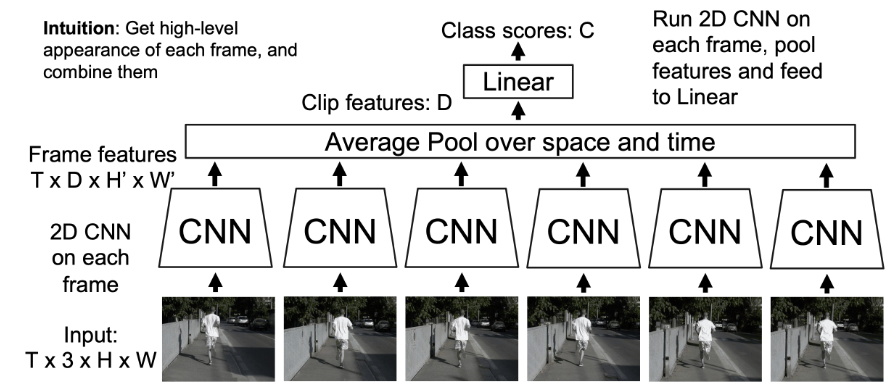
\includegraphics[scale=0.25]{figures/LF_pool.png}
    \caption{Late Fusion with Pooling}
\end{figure}

看得出来正着走和倒着走的区别吗? 看不出来

看得出来跑和走的区别吗? 看得出来,分辨重心feature.

更好得区分跑和走? 使用MaxPool, 在fusion的时候不要模糊所有帧的特征

\subsection{Video Classification: Early Fusion}

\begin{figure}[htbp]
    \centering
    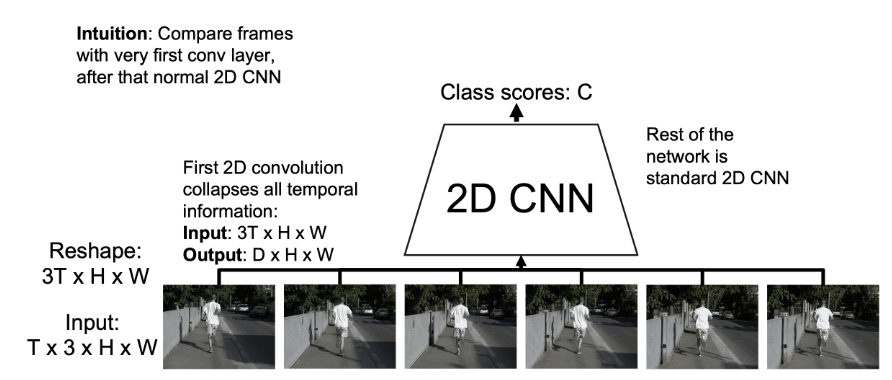
\includegraphics[scale=0.25]{figures/EF.png}
    \caption{Early Fusion}
\end{figure}

early fusion:所有时间信息在第一步提取,难度较高

所以一层处理时间信息可能不够

\subsection{Video Classification: 3D CNN}

\begin{figure}[htbp]
    \centering
    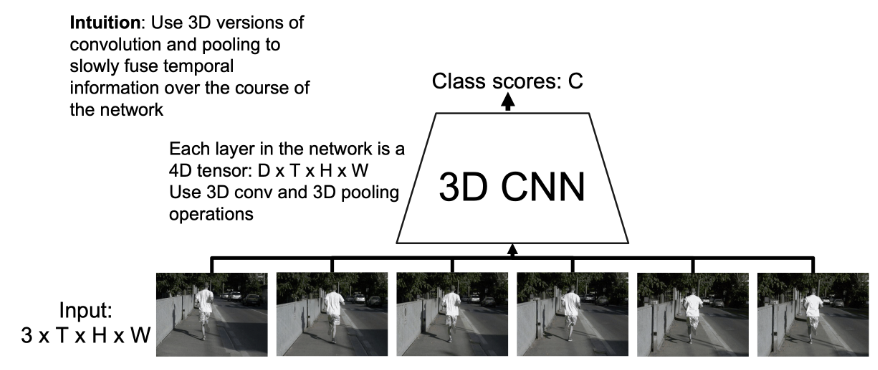
\includegraphics[scale=0.25]{figures/3DCNN.png}
    \caption{3D CNN}
\end{figure}

3D CNN将时间视作第三个空间维度.但问题在于:这对感受野的要求比较大.在视频当中,
一件事情的效应可能在相当长的时间之后才能体现,
但CNN也不可能cover任意长的时间序列.也就是说,在视频处理当中,
空间范围和时间范围地位并不对等.

3D CNN在各个维度感受野的增长比较均匀.

\subsection{Comparison}

\begin{figure}[htbp]
    \centering
    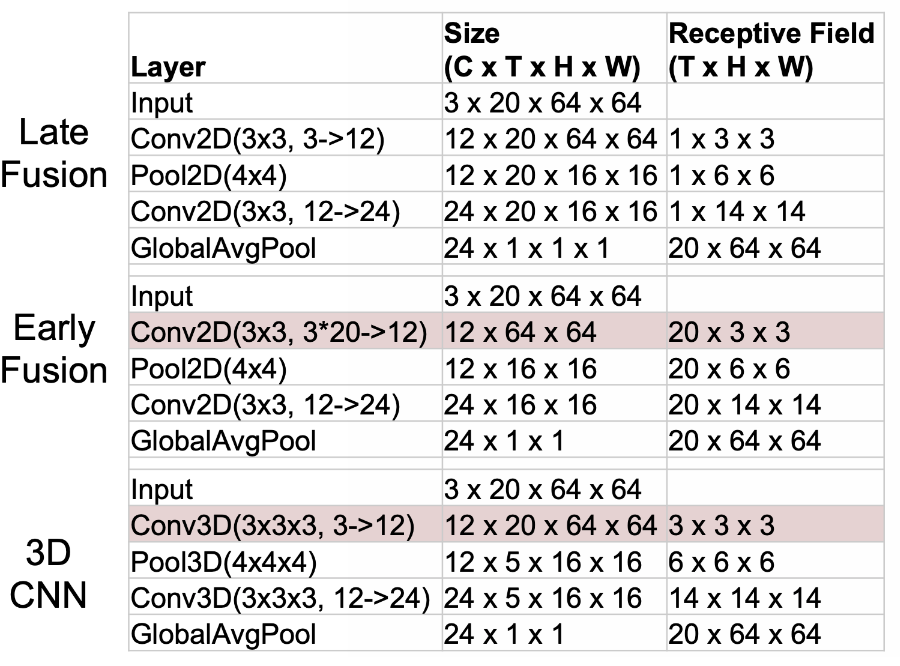
\includegraphics[scale=0.35]{figures/video_cmp.png}
    \caption{Video analysis method comparison}
\end{figure}

3D CNN 与 2D CNN 相比, 把卷积核扩展到时间维度, 感受野在时间维度上也是逐渐增大的.

\begin{itemize}
    \item Late Fusion: Build slowly in space, All-at-once in time at end
    \item Early Fusion: Build slowly in space, All-at-once in time at start
    \item 3D CNN: Build slowly in space, Build slowly in time "Slow Fusion"
\end{itemize}

\subsection{C3D: The VGG of 3D CNNs}

C3D: The VGG of 3D CNNs.第一次pool没有在时间维上处理,不希望提取得太早.

3d的kernel size比较敏感,$5^3 > 11^2$.移动多了一个维度,计算代价更大.得益于其网络的精良设计,C3D的 sports-1m 的top5 acc还是达到了84\%.

人类识别运动的关键:Motion,不是pixel.

Use Both Motion and appearance: two-stream fusion network.它使用经典算法获得flow输入神经网络.神经网络分为两支,一支做空间,一支做时间.时间(flow)这一支使用了early fusion,因为相对于RGB,光流的信息已经比较清晰.

\subsection{Modeling Long-Term Temporal Structure}

我们希望处理序列,RNN如何? aggregation(聚合).

CNN和RNN一起训练计算代价太大\marginpar{\kaishu 原来RNN是独立的网络吗?}.
因此先train CNN,不向其传递梯度,只训练RNN.但这样CNN与RNN可能优化目标不同.

如何 pre-train? 使用ImagenNet不好, 因为ImageNet的分类和Sports1M的分类粒度不同.

end to end training:端到端训练.所有optimization variable同时被优化.

\subsection{Recurrent convolutional Network}

\begin{figure}[htbp]
    \centering
    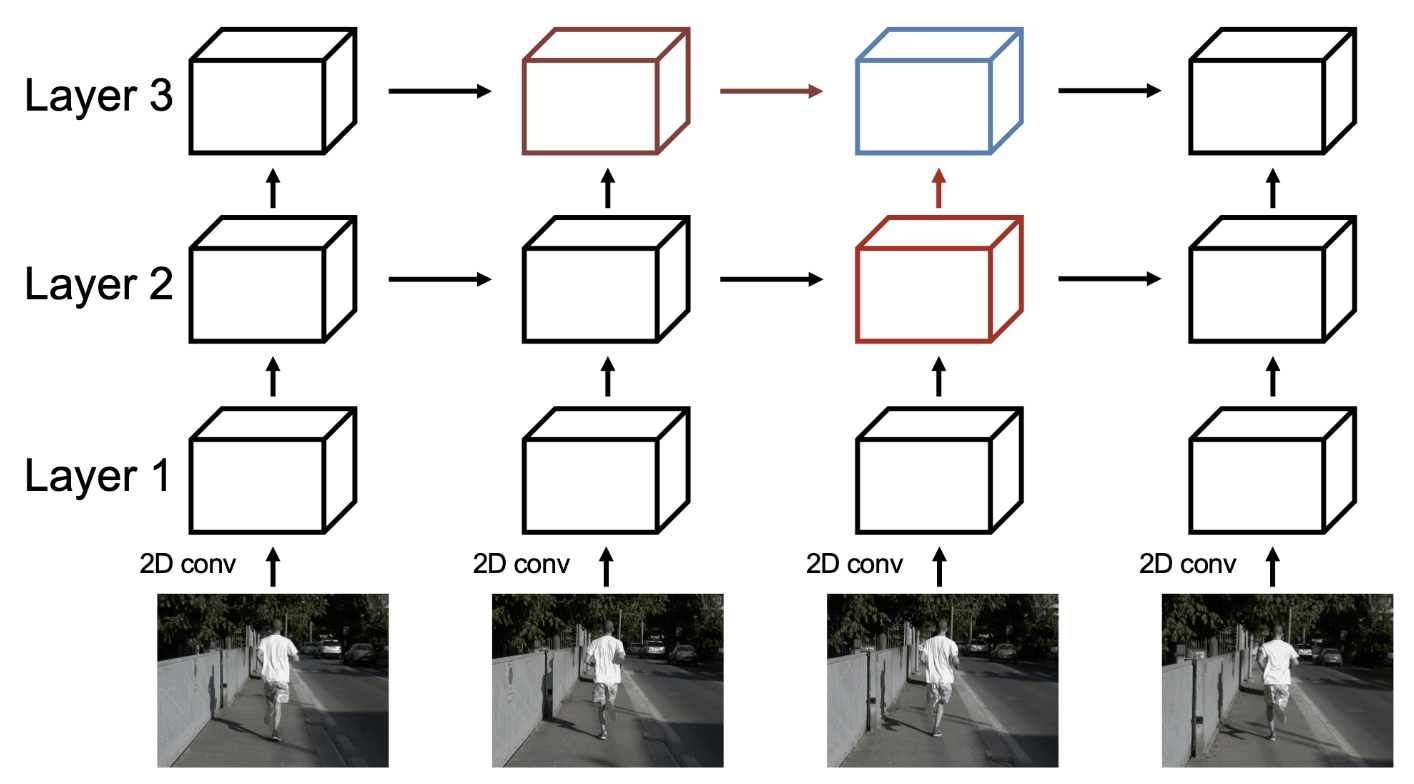
\includegraphics[scale=0.25]{figures/recu_CNN.png}
    \caption{Recurrent convolutional Network}
\end{figure}

跟 3D CNN 区别: 3D CNN 不是 recurrent 的, 是被3D卷积核决定的一个固定长度, 
而 recurrent convolutional network 是一个 recurrent network, 可以读取到之前所有的信息.
